\documentclass[a4paper]{book}
% chktex-file 
% chktex-file 3
\usepackage{geometry}
% make full use of A4 papers
\geometry{margin=1.5cm, vmargin={0pt,1cm}}
\setlength{\topmargin}{-1cm}
\setlength{\paperheight}{29.7cm}
\setlength{\textheight}{25.1cm}

% auto adjust the marginals
\usepackage{marginfix}

\usepackage{amsfonts}
\usepackage{amsmath}
\usepackage{amssymb}
\usepackage{amsthm}
% \usepackage{CJKutf8}   % for Chinese characters
\usepackage{ctex}
\usepackage{enumerate}
\usepackage{graphicx}  % for figures
\usepackage{layout}
\usepackage{multicol}  % multiple columns to reduce number of pages
\usepackage{mathrsfs}
\usepackage{fancyhdr}
\usepackage{subfigure}
\usepackage{tcolorbox}
\usepackage{tikz-cd}
\usepackage{listings}
\usepackage{xcolor} %代码高亮
\usepackage{braket}
% ------------------
% common commands %
% ------------------
% differentiation
\newcommand{\gen}[1]{\left\langle#1 \right\rangle}
\newcommand{\dif}{\mathrm{d}}
\newcommand{\difPx}[1]{\frac{\partial#1}{\partial x}}
\newcommand{\difPy}[1]{\frac{\partial#1}{\partial y}}
\newcommand{\Dim}{\mathrm{D}}
\newcommand{\avg}[1]{\left\langle#1 \right\rangle}
\newcommand{\sgn}{\mathrm{sgn}}
\newcommand{\Span}{\mathrm{span}}
\newcommand{\dom}{\mathrm{dom}}
\newcommand{\Arity}{\mathrm{arity}}
\newcommand{\Int}{\mathrm{Int}}
\newcommand{\Ext}{\mathrm{Ext}}
\newcommand{\Cl}{\mathrm{Cl}}
\newcommand{\Fr}{\mathrm{Fr}}
% group is generated by
\newcommand{\grb}[1]{\left\langle#1 \right\rangle}
% rank
\newcommand{\rank}{\mathrm{rank}}
\newcommand{\Iden}{\mathrm{Id}}

% this environment is for solutions of examples and exercises
\newenvironment{solution}%
{\noindent\textbf{Solution.}}%
{\qedhere}
% the following command is for disabling environments
% so that their contents do not show up in the pdf.
\makeatletter
\newcommand{\voidenvironment}[1]{%
  \expandafter\providecommand\csname env@#1@save@env\endcsname{}%
  \expandafter\providecommand\csname env@#1@process\endcsname{}%
  \@ifundefined{#1}{}{\RenewEnviron{#1}{}}%
}
\makeatother

% ---------------------------------------------
% commands specifically for complex analysis %
% ---------------------------------------------
% complex conjugate
\newcommand{\ccg}[1]{\overline{#1}}
% the imaginary unit
\newcommand{\ii}{\mathbf{i}}
% \newcommand{\ii}{\boldsymbol{i}}
% the real part
\newcommand{\Rez}{\mathrm{Re}\,}
% the imaginary part
\newcommand{\Imz}{\mathrm{Im}\,}
% punctured complex plane
\newcommand{\pcp}{\mathbb{C}^{\bullet}}
% the principle branch of the logarithm
\newcommand{\Log}{\mathrm{Log}}
% the principle value of a nonzero complex number
\newcommand{\Arg}{\mathrm{Arg}}
\newcommand{\Null}{\mathrm{null}}
\newcommand{\Range}{\mathrm{range}}
\newcommand{\Ker}{\mathrm{ker}}
\newcommand{\Iso}{\mathrm{Iso}}
\newcommand{\Aut}{\mathrm{Aut}}
\newcommand{\ord}{\mathrm{ord}}
\newcommand{\Res}{\mathrm{Res}}
% \newcommand{\GL2R}{\mathrm{GL}(2,\mathbb{R})}
\newcommand{\GL}{\mathrm{GL}}
\newcommand{\SL}{\mathrm{SL}}
\newcommand{\Dist}[2]{\left|{#1}-{#2}\right|}

\newcommand\tbbint{{-\mkern-16mu\int}}
\newcommand\tbint{{\mathchar'26 -\mkern-14mu\int}}
\newcommand\dbbint{{-\mkern-20mu\int}}
\newcommand\dbint{{\mathchar'26 -\mkern-26mu\int}}
\newcommand\bint{
  {\mathchoice{\dbint}{\tbint}{\tbint}{\tbint}}
}
\newcommand\bbint{
  {\mathchoice{\dbbint}{\tbbint}{\tbbint}{\tbbint}}
}





% ----------------------------------------
% theorem and theorem-like environments %
% ----------------------------------------
\numberwithin{equation}{chapter}
\theoremstyle{definition}

\newtheorem{thm}{Theorem}[chapter]
\newtheorem{axm}[thm]{Axiom}
\newtheorem{alg}[thm]{Algorithm}
\newtheorem{asm}[thm]{Assumption}
\newtheorem{defn}[thm]{Definition}
\newtheorem{prop}[thm]{Proposition}
\newtheorem{rul}[thm]{Rule}
\newtheorem{coro}[thm]{Corollary}
\newtheorem{lem}[thm]{Lemma}
\newtheorem{exm}{Example}[chapter]
\newtheorem{rem}{Remark}[chapter]
\newtheorem{exc}[exm]{Exercise}
\newtheorem{frm}[thm]{Formula}
\newtheorem{ntn}{Notation}

% for complying with the convention in the textbook
\newtheorem{rmk}[thm]{Remark}


% \lstset{
%	backgroundcolor=\color{red!50!green!50!blue!50},%代码块背景色为浅灰色
%	rulesepcolor= \color{gray}, %代码块边框颜色
%	breaklines=true,  %代码过长则换行
%	numbers=left, %行号在左侧显示
%	numberstyle= \small,%行号字体
%	keywordstyle= \color{blue},%关键字颜色
%	commentstyle=\color{gray}, %注释颜色
%	frame=shadowbox%用方框框住代码块
% }
\lstset{
  columns=fixed,
  numbers=left,                                        % 在左侧显示行号
  numberstyle=\tiny\color{gray},                       % 设定行号格式
  frame=none,                                          % 不显示背景边框
  backgroundcolor=\color[RGB]{245,245,244},            % 设定背景颜色
  keywordstyle=\color[RGB]{40,40,255},                 % 设定关键字颜色
  numberstyle=\footnotesize\color{darkgray},
  commentstyle=\it\color[RGB]{0,96,96},                % 设置代码注释的格式
  stringstyle=\rmfamily\slshape\color[RGB]{128,0,0},   % 设置字符串格式
  showstringspaces=false,                              % 不显示字符串中的空格
  language=c++,                                        % 设置语言
}

% ----------------------
% the end of preamble %
% ----------------------

\begin{document}
\pagestyle{empty}
\pagenumbering{roman}
% 
% \tableofcontents
% \clearpage

% \pagestyle{fancy}
% \fancyhead{}
% \lhead{Qinghai Zhang}
% \chead{Notes on Algebraic Topology}
% \rhead{Fall 2018}


\setcounter{chapter}{5}
\pagenumbering{arabic}
% \setcounter{page}{0}

% --------------------------------------------------------
% uncomment the following to remove these environments
% to generate handouts for students.
% --------------------------------------------------------
% \begingroup
% \voidenvironment{rem}%
% \voidenvironment{proof}%
% \voidenvironment{solution}%


% each chapter is factored into a separate file.

\chapter{Homework 21935004 谭焱}
% \begin{lstlisting}
%   int main(){
%   double d;
%   int i;
%   return i;
% }
% \end{lstlisting}
% The main ingredients of snacks are sugar and fat;
% the main ingredients of math are logic and set theory.


%\begin{multicols}{2}
% \setlength{\columnseprule}{0.2pt}

\begin{exc}
  2.  Compute the envelopes of the family of lines
  \begin{equation}
    \label{eq:6:1:1}
    x_1 + a^2 x_2 - 2a = 0 \qquad (a \in \mathbb{R})
  \end{equation}
  in $\mathbb{R}^2$ and of the family of planes
  \begin{equation}
    \label{eq:6:1:2}
    2 a_1 x_1 + 2 a_2 x_x - x_3 + a_1^2 + a_2^2 = 0 \qquad (a_1, a_2 \in \mathbb{R})
  \end{equation}
  in $\mathbb{R}^3$. Draw pictures illustrating the geometric meaning of the enveplopes.
\end{exc}

\begin{solution}
  Let $u(x,a) = x_1 + a^2 x_2 - 2a $, from definition of envelopes
  \begin{align*}
    &D_a u = 2 a x_2 - 2 = 0 \Longrightarrow \\
    &a = \frac{1}{x_2}.
  \end{align*}
  So envelopes is $x_1 - \frac{1}{x_2} = 0$.

  Similarly,
  \begin{align*}
    &2 x_1 + 2 a_1 = 0 \Longrightarrow a_1 = - x_1 \\
    &2 x_2 + 2 a_2 = 0 \Longrightarrow a_2 = - x_2 \\
    &\Longrightarrow \mathbf{a} = - \mathbf{x}
  \end{align*}
  So envelopes is $ x_1^2 + x_2^2 - x_3 = 0$.

  Above envelopes in $\mathbb{R}^2$ ploted blow
  \begin{figure}
    \centering
    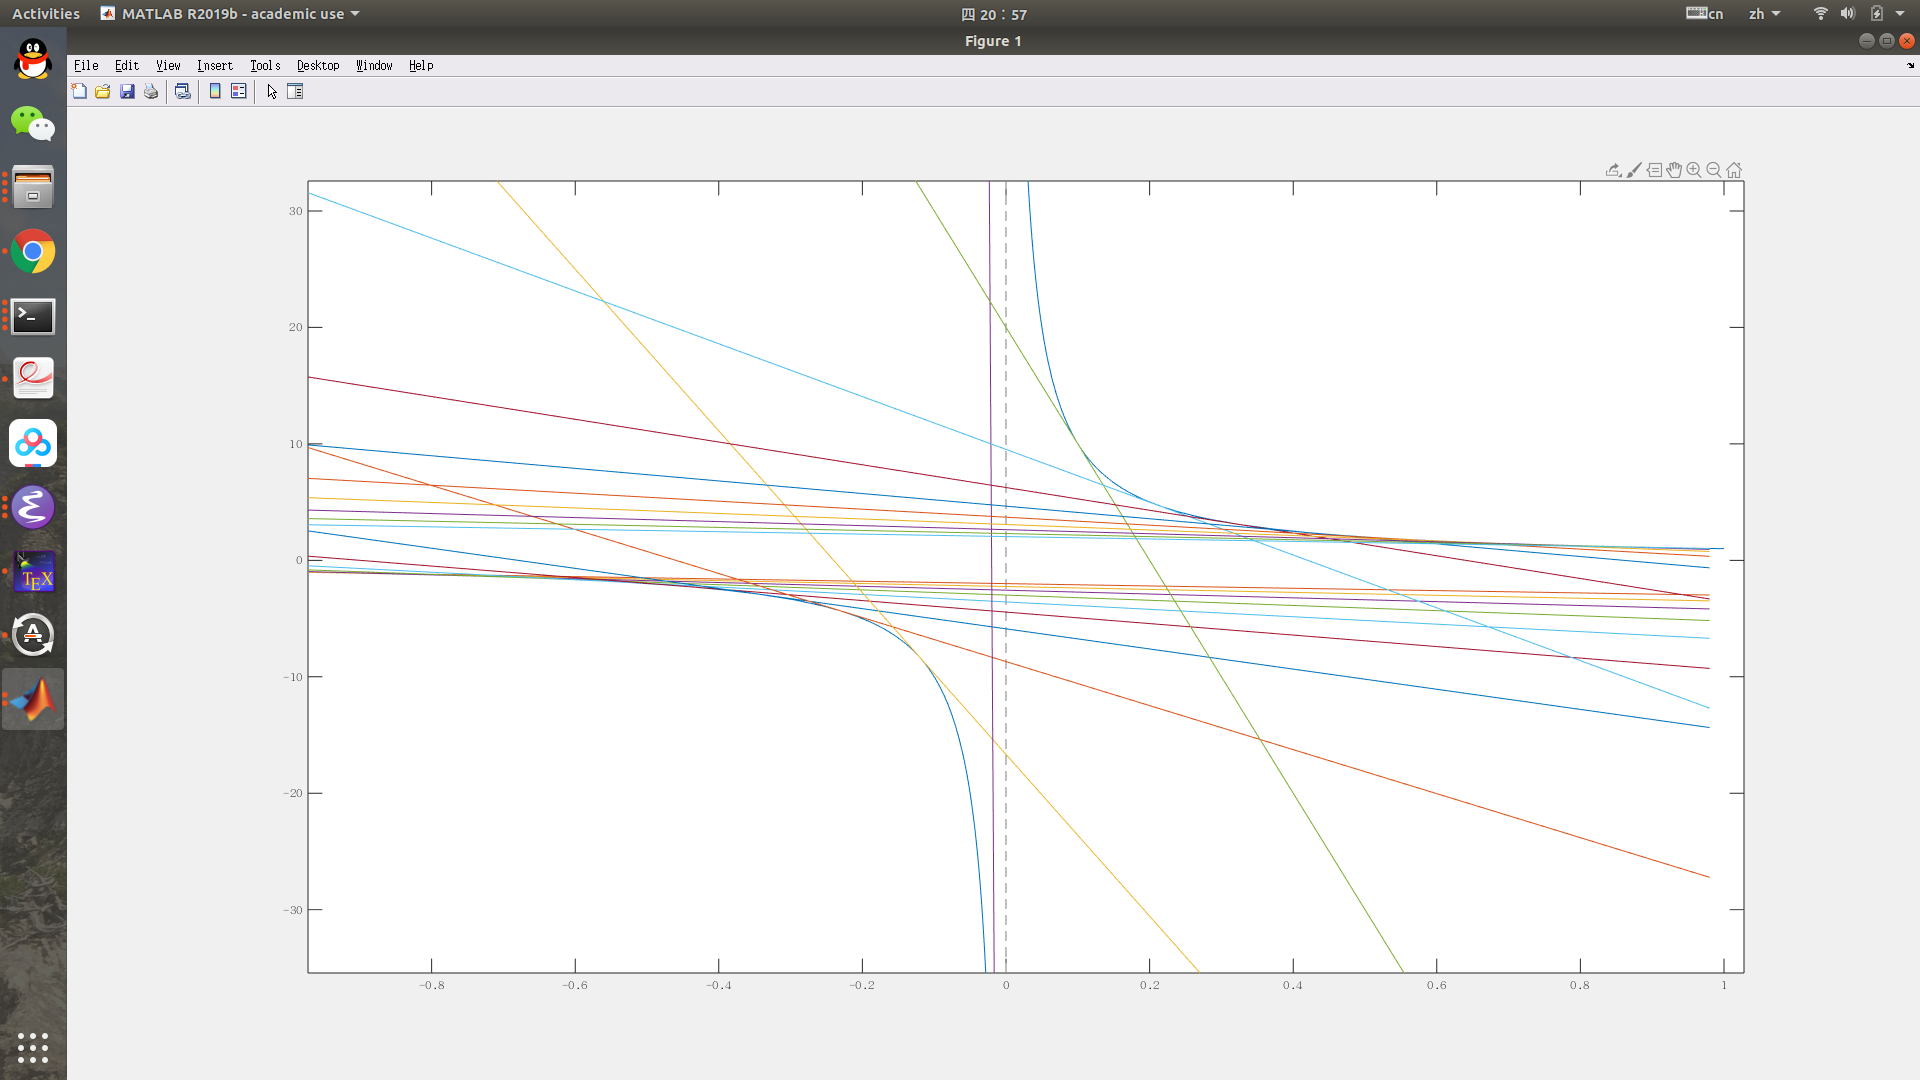
\includegraphics[scale = 0.2]{2.png}
    \caption{envelopes}\label{fig:6:1:1}
  \end{figure}
  envelopes is all point \textit{x} satisfy that exist a line \textit{u} in the family such that $u(x) = 0$. 
\end{solution}


\begin{exc}
  4.  
  \begin{enumerate} [(a)]
  \item  Write down the characteristic equations for the PDE
    \begin{equation} \nonumber
      u_t + b \cdot Du = f \qquad \textmd{in } \mathbb{R}^n \times (0, \infty), \leqno(*)
    \end{equation}
    where $b \in \mathbb{R}^n, f = f(x,t)$.

  \item Use the characteristic ODE to solve $(*)$ subject to the initial condition
    \begin{equation}
      \label{eq:6:3:1}
      u = g \qquad \textmd{on } \mathbb{R}^n \times \{t = 0\}.
    \end{equation}
    Make sure your answer agrees with formula (5) in 2.1.2.
  \end{enumerate}
\end{exc}

\begin{solution}
  \begin{enumerate}[(a)]
  \item Transfer (*) to $\mathbf{F}(\mathbf{p}(s),z(s),\mathbf{x}(s)) = (b,1)\cdot\mathbf{p}(s) - f(\mathbf{x}) = 0 $, then
    \begin{align*}
      &\dot{\mathbf{p}}(s) = - (D_x f(\mathbf{x},t) + D_t f(\mathbf{x},t)) \\
      &\dot{z}(s) = (b,1) \cdot \mathbf{p}(s) \\
      &\dot{\mathbf{x}}(s) = (b,1) \\
    \end{align*}

  \item Solving second and third of the equations get
    \begin{align*}
      &\mathbf{x}(s) = (bs,s) + (x_0,0) \\
      &\dot{z}(s) = f(\mathbf{x}) \Longrightarrow \\
      &z(s) = \int_0^t f((bs + x_0,s))ds + g(x_0) \\
     % &z(s) = \int_0^t f((x + (s -t)b, s))ds + g(x_0)
    \end{align*}
    Since $\mathbf{x}(s) = (bs,s) + (x_0,0)$, eliminating the $x_0$ in last equaltion get the formula (5). 
  \end{enumerate}
\end{solution}

\begin{exc}
  5.  Solve using characteristic:
  \begin{enumerate} [(a)]
  \item
    \begin{equation}
      \label{eq:6:4:1}
      x_1 u_{x_1} + 2 x_2 u_{x_2} + u_{x_3} = 3u, \qquad u(x_1, x_2, 0) = g(x_1, x_2).
    \end{equation}

    \item
      \begin{equation}
        \label{eq:6:4:2}
        u u_{x_1} + u_{x_2} = 1, \qquad u(x_1, x_1) = \frac{1}{2} x_1.
      \end{equation}

  \end{enumerate}
\end{exc}

\begin{solution}
  \begin{enumerate} [(a)]
  \item Writing characterstic equations as follow
    \begin{align*}
      &F(\mathbf{p}(s), z(s), \mathbf{x}(s)) = (x_1,2x_2,1) \cdot \mathbf{p}(s) - 3 z(s) = 0 \\
     % &\dot{\mathbf{p}}(s) = - 3 \mathbf{p}(s) \\
      &\dot{z}(s) = 3 z(s) \\
      &\dot{\mathbf{x}}(s) = (x_1, 2 x_2, 1) 
    \end{align*}
    Solving equations get $\mathbf{x}(s) = (x^0_1e^{s},x^0_2e^{2s},s), z(s) = z^0 e^{3s}$, eliminating $x^0_1,x^0_2,z^0$ to obtain $u(x_1,x_2,x_3) = g(\frac{x_1}{e^{x_3}}, \frac{x_2}{e^{x_3}}) e^{3s}$.

    \item
      \begin{align*}
        &F(\mathbf{p}(s), z(s), \mathbf{x}(s)) = (z(s),1) \cdot \mathbf{p}(s) - 1 = 0 \\
       % &\dot{\mathbf{p}}(s) = (z(s),1) \\
        &\dot{z}(s) = 1 \\
        &\dot{\mathbf{x}}(s) = (z(s),1).
      \end{align*}
      Solving equations get $z(s) = s + z_0, \mathbf{x}(s) = (\frac{1}{2}s^2 + z_0 s + x^0_1, s + x^0_2)$. By $u(x_1,x_1) = \frac{1}{2}x_1 \Longrightarrow z_0 = \frac{1}{2}x^0_1 = \frac{1}{2}x^0_2$, eliminating $z_0,x^0_1,x^0_2$ obtain $u(x_1,x_2) = \frac{1}{2}x_2 + \frac{x_2 - x_1}{2 - x_2}$.
  \end{enumerate}
\end{solution}

\begin{exc}
  6.  Given a smooth vector field \textbf{b} on $\mathbb{R}^n$, let $\mathbf{x}(s) = \mathbf{x}(s,x,t)$ solve the ODE
  \begin{eqnarray} \nonumber
    \begin{cases}
      \dot{\mathbf{x}} = \mathbf{b}(x) \qquad (s \in \mathbb{R}) \\
      \mathbf{x}(t) = x.
    \end{cases}
  \end{eqnarray}
  \begin{enumerate}[(a)]
  \item Define the Jacobian
    \begin{equation}
      \label{eq:6:5:1}
      J(s,x,t) := \det D_x\mathbf{x}(s,x,t)
    \end{equation}
    and derive \textit{Euler's formula}:
    \begin{equation}
      \label{eq:6:5:2}
      J_s = \textmd{div}\, \mathbf{b(x)}J.
    \end{equation}

  \item Demonstrate that
    \begin{equation}
      \label{eq:6:5:3}
      u(x,t) := g(\mathbf{x}(0,x,t))J(0,x,t)
    \end{equation}
    solves
    \begin{eqnarray}
      \label{eq:6:5:4}
      \begin{cases}
        \begin{aligned}
        u_t + \textmd{div}\,(u\mathbf{b}) &= 0 \qquad \textmd{in } \mathbb{R}^n \times (0,\infty) \\
        u &= g \qquad \textmd{on } \mathbb{R}^n \times \{t = 0\},
        \end{aligned}
      \end{cases}
    \end{eqnarray}
    (Hint: Show $\frac{\partial}{\partial s}(u(\mathbf{x},s)J) = 0$.)
  \end{enumerate}
\end{exc}

\begin{solution}
  \begin{enumerate} [(a)]
  \item Unfold $J$ and differential $J$
    \begin{align*}
      J(s,x,t) &= \sum \prod_{i = 1}^n (-1)^{\sigma} x^i_{\sigma(i)} \\
      J_s &= \sum \sum_{j = 1}^n (\prod_{i \neq j} (-1)^{\sigma} x^i_{\sigma(i)}) x^j_{\sigma(j) s}  \\
               &= \sum \sum _{j = 1}^n (\prod_{i=1}^n (-1)^{\sigma} x^i_{\sigma(i)}) (\mathbf{b}^j(x)(s -t) + x)_{\sigma(j)s} \\
               &=  \sum \sum _{j = 1}^n (\prod_{i=1}^n (-1)^{\sigma} x^i_{\sigma(i)}) \mathbf{b}^j_j(x)x^j_{\sigma(j)}  \\
      &= \textmd{div}\, \mathbf{b}(x)J.
    \end{align*}

  \item Boundary condition is obvious, since $J(0,x,0) = \det D_x x(0,x,0) = \det D_x x = 1 \textmd{ and } x(0,x,0) = x$.And $g(\mathbf{x}) J$ means that transfer coordinate$\mathbf{x}(s,x,t)$ to $\mathbf{x}$. So it value $u(x,t)$ won't change while $\mathbf{x}$ is constant.It follows that $0 = \frac{\partial}{\partial s}(u(\mathcal{x},s)J) = u_t(x,s)J + u(x,s)J_s = u_t(x,s)J + u(x,s)\textmd{div}\, (\mathbf{b}J) = (u_t + \textmd{div}\, (u\mathbf{b}))J = 0$.We know that $J$ won't be zero when $t = s$, therefore (\ref{eq:6:5:4}) is solved by $u(x,t)$.
  \end{enumerate}
\end{solution}

\begin{exc}
  8.  Confirm that the formula $u = g(x - t \mathbf{F}^\prime (u))$ from 3.2.5 provides an implicit solution for the conservation law
  \begin{equation}
    \label{eq:6:6:1}
    u_t + \mathbf{F}(u)_x = 0.
  \end{equation}
\end{exc}

\begin{solution}
  The initial condition is trival, then confirm the function
  \begin{align*}
    &u_t + \mathbf{F}(u)_x = 0 \Longleftrightarrow \\
    &u_t = D g \cdot (x - t\mathbf{F}^\prime(u))(- \mathbf{F}^\prime(u) - t \mathbf{F}^{\prime \prime}(u) u_t) \textmd{ While } 1 + t \mathbf{F}^{\prime \prime}(u) \neq 0 \\
    &u_t = - \frac{D g \cdot \mathbf{F}^\prime(u)}{1 + D g \cdot t \mathbf{F}^{\prime \prime}(u)} \\
    &\mathbf{F}(u)_x = D \mathbf{F}(u) = \mathbf{F}^\prime(u) \cdot D u \\
    &\frac{\partial}{\partial x_i} u = \frac{\partial}{\partial x_i} g(x - t \mathbf{F}^\prime (u)) \\
    &\qquad \; = g_{x_i} (1 - t \mathbf{F}^{\prime \prime}(u) \cdot u_{x_i}) \textmd{ need the same requirement above so that } \\
    &D u = \frac{D g}{1 + t \mathbf{F}^{\prime \prime}(u)} \\
    &u_t - \mathbf{F}^\prime(u) \cdot D u = 0
  \end{align*}
\end{solution}




  % \section{1}
  % \label{sec:logic}
  % \begin{defn}
  A \emph{set} ${\cal S}$
  is a collection of \emph{distinct} objects $x$'s,
   often denoted with the following notation
   \begin{equation}
     \label{eq:setNotation}
     {\cal S} = \{ x\ |\ \text{ the conditions that $x$ satisfies. } \}.
   \end{equation}
\end{defn}

\begin{ntn}
$\mathbb{R}, \mathbb{Z}, \mathbb{N}, \mathbb{Q}, \mathbb{C}$
 denote 
 the sets of real numbers, integers, natural numbers,
 rational numbers and complex numbers, respectively.
$\mathbb{R}^+, \mathbb{Z}^+, \mathbb{N}^+, \mathbb{Q}^+$
 the sets of positive such numbers.
\end{ntn}

 \begin{defn}
   ${\cal S}$ is a \emph{subset} of ${\cal U}$,
    written as ${\cal S}\subseteq {\cal U}$,
   if and only if (iff) $x\in {\cal S}$ $\Rightarrow$ $x\in {\cal U}$.
   ${\cal S}$ is a \emph{proper subset} of ${\cal U}$,
    written as ${\cal S}\subset {\cal U}$,
    if ${\cal S}\subseteq {\cal U}$
    and $\exists x\in {\cal U}$ s.t. $x\not\in{\cal S}$.
 \end{defn}

\begin{defn}[Statements of first-order logic]
\label{def:uni_exist}
A \emph{universal statement} is a logic statement 
 of the form
\begin{equation}
  \mathsf{U} = (\forall x\in {\cal S},\ \mathsf{A}(x) ).
\end{equation}
An \emph{existential statement} has the form
\begin{equation}
  \mathsf{E} = (\exists x\in {\cal S},\text{ s.t. } \mathsf{A}(x)),
\end{equation}
 where 
 $\forall$ (``for each'') and $\exists$ (``there exists'')
 are the \emph{quantifiers}, ${\cal S}$ is a set,
 ``s.t.'' means ``such that,''
 and $\mathsf{A}(x)$ is the \emph{formula}.\\
A statement of \emph{implication/conditional}
 has the form
 \begin{equation}
   \mathsf{A}\Rightarrow \mathsf{B}.
 \end{equation}
\end{defn}

 \begin{exm}
   Universal and existential statements:\\
   $\forall x\in[2,+\infty)$, $x>1$;\\
   $\forall x\in \mathbb{R}^+$, $x>1$;\\
   $\exists p,q\in \mathbb{Z}, \text{ s.t. } p/q = \sqrt{2}$;\\
   $\exists p,q\in \mathbb{Z}, \text{ s.t. } \sqrt{p} = \sqrt{q}+1$.
 \end{exm}

\begin{defn}
  \emph{Uniqueness quantification}
   or \emph{unique existential quantification},
   written $\exists!$ or $\exists_{=1}$, 
   indicates that exactly one object with a certain property exists.
\end{defn}

\begin{exc}
  Express the logic statement $\exists! x, \text{ s.t. } \mathsf{A}(x)$
   with $\exists$, $\forall$, and $\Leftrightarrow$.
\end{exc}
\begin{solution}
  $\exists x \text{ s.t. }\forall y, \mathsf{A}(y) \Leftrightarrow x=y.$
\end{solution}

 \begin{rem}
A logic statement is either true or false.
There is no such thing that
 a logic statement is sometimes true and sometimes false.
To prove a universal statement,
 conceptually we have to verify the statement
 for all elements in the set.
To deny a universal statement,
 we only need to show a counterexample.
To prove an existential statement,
 we only need to show an instance.
To deny an existential statement,
 conceptually we have to show that the statement holds
 for none of the elements.
 \end{rem}

 \begin{rem}
   In Definition \ref{def:uni_exist},
    the formula $\mathsf{A}(x)$ itself
    might also be a logic statement.
   Hence universal and existential statements
    might be nested.
   This observation leads to the next definition.
 \end{rem}

 \begin{defn}
   A \emph{universal-existential statement} is a logic statement 
   of the form
   \begin{equation}
     \mathsf{U}_E =
     (\forall x\in {\cal S},\ \exists y\in {\cal T}
     \text{ s.t. } \mathsf{A}(x,y)).
   \end{equation}
   An \emph{existential-universal statement} has the form
   \begin{equation}
     \mathsf{E}_U =
     (\exists y\in {\cal T},\text{ s.t. } \forall x\in {\cal S},\ 
     \mathsf{A}(x,y)).
   \end{equation}
 \end{defn}

 \begin{exm}
   True or false:\\
   $\forall x\in[2,+\infty)$, $\exists y\in \mathbb{Z}^+$ s.t. $x^y<10^5$;\\
   $\exists y\in \mathbb{R}$ s.t.
   $\forall x\in[2,+\infty)$, $x>y$;\\
   $\exists y\in \mathbb{R}$ s.t.
   $\forall x\in[2,+\infty)$, $x<y$.
 \end{exm}

\begin{exc}
  [Translating an English statement into a logic statement]
  Goldbach's conjecture states
   \emph{every even natural number greater than 2
     is the sum of two primes}.
 \end{exc}
\begin{solution}
  Let $\mathbb{P}\subset \mathbb{N}^+$
   denote the set of prime numbers.
  Then Goldbach's conjecture is
  \begin{displaymath}
  \forall a\in 2\mathbb{N}^++2,
   \exists p,q\in \mathbb{P} \text{ s.t. } a=p+q.\qedhere
  \end{displaymath}
\end{solution}

\begin{thm}
   The existential-universal statement
    implies the corresponding universal-existential statement,
    but not vice versa.
 \end{thm}

 \begin{exm}[Translating a logic statement to an English statement]
   Let ${\cal S}$ be the set of all human beings.\\
   $U_E=$($\forall p\in{\cal S}, \exists q\in{\cal S}$ s.t. $q$ is $p$'s mom.)
   \\
   $E_U$=( $\exists q\in{\cal S}$ s.t.
   $\forall p\in{\cal S}, $ $q$ is $p$'s mom.)\\
   $U_E$ is probably true, but $E_U$ is certainly false. \\
   If $E_U$ were true, then $U_E$ would be true. why?
 \end{exm}

\begin{axm}[First-order negation of logical statements]
  The negations of the statements in Definition \ref{def:uni_exist}
  are
  \begin{align}
  \neg \mathsf{U} &= (\exists x\in {\cal S},\text{ s.t. }
  \neg \mathsf{A}(x)).
  \\
  \neg \mathsf{E} &= (\forall x\in {\cal S},\ 
  \neg \mathsf{A}(x)).
  \end{align}
\end{axm}

\begin{rul}
  The negation of a more complicated logic statement
   abides by the following rules:
\begin{itemize}\itemsep0em
\item switch the type of each quantifier until
  you reach the last formula without quantifiers;
\item negate the last formula.
\end{itemize}
  One might need to group quantifiers of like type.
\end{rul}

\begin{exc}
  Write the logic statement
   for the negation of Goldbach's conjecture.
\end{exc}
\begin{solution}
  $\exists a\in 2\mathbb{N}^++2$ s.t. $\forall p,q \in \mathbb{P}$, 
   $a\ne p+q$.
\end{solution}

   % \begin{exc}
   %   A weaker version of Goldbach's conjecture states
   %   \emph{Goldbach's conjecture has
   %     at most a finite number of of counterexamples}.
   %   Formulate it into a logical statement
   %    with explicit quatifiers.
   % \end{exc}

   % \begin{exc}
   %   The only even prime is 2.\\
   %   Multiplication of integers is associative. \\
   %   Every positive integer has a unique prime factorization.
   % \end{exc}

\begin{axm}[Contraposition]
  \label{axm:contrapositive}
  A conditional statement is logically equivalent to its
  contrapositive.
  \begin{equation}
    \label{eq:contraposition}
    (\mathsf{A}\Rightarrow \mathsf{B}) \Leftrightarrow
    (\neg \mathsf{B}\Rightarrow \neg \mathsf{A})
  \end{equation}
\end{axm}

\begin{exm}
  \label{exm:contrapositive}
  ``If Jack is a man, then Jack is a human being.''
  is equivalent to ``If Jack is not a human being,
  then Jack is not a man.''
\end{exm}

\begin{exc}
  Draw an Euler diagram of subsets to illustrate Example \ref{exm:contrapositive}.
\end{exc}

%%% Local Variables:
%%% mode: latex
%%% TeX-master: "../notesAlgebraicTopology"
%%% End:


  % \section{Ordered sets}
  % \label{sec:sets}
  % \begin{defn}
  The \emph{Cartesian product} ${\cal X}\times {\cal Y}$
   between two sets ${\cal X}$ and ${\cal Y}$
   is the set of all possible ordered pairs with first element
   from ${\cal X}$ and second element from ${\cal Y}$:
   \begin{equation}
     {\cal X}\times {\cal Y} = \{(x,y)\ |\ x\in {\cal X},\ y\in {\cal Y}\}.
   \end{equation}
\end{defn}

\begin{axm}[Fundamental principle of counting]
  \label{axm:multiplicationPrinciple}
  A task consists of a sequence of $k$ independent steps.
  Let $n_i$ denote the number of different choices for the $i$-th step,
   the total number of distinct ways to complete the task
   is then
   \begin{equation}
     \prod_{i=1}^{k} n_i = n_1n_2\cdots n_k.
   \end{equation}
 \end{axm}

 \begin{exm}
   \label{exm:dinnerCombo}
   Let $A, E, D$ be the set of appetizers,
    main entrees, desserts in a restaurant.
   $A\times E\times D$
    is the set of possible dinner combos.
   If $\#A=10$, $\#E=5$, $\#D=6$,
    $\#(A\times E\times D)=300$.
 \end{exm}

 \begin{rem}
   The menu of a restaurant in Example \ref{exm:dinnerCombo}
    seldom contains all the different combinations
    explicitly spelled out.
   You simply pick one entry from each category
    and call the three choices your own dinner.
   In math learning,
    you follow a similar pattern.
   You learn algebra and topology,
    then you combine the two to learn algebraic topology.
   The difference is that,
    the process of coupling the two is much more difficult
    and much more powerful.
 \end{rem}

% \begin{defn}[Maximum and minimum]
%   Consider ${\cal S}\subseteq \mathbb{R}$,
%    ${\cal S}\ne \emptyset$.
%   If $\exists s_m\in{\cal S}$
%    s.t. $\forall x\in {\cal S}$, $x\le s_m$,
%    then $s_m$ is the \emph{maximum} of ${\cal S}$
%    and denoted by $\max {\cal S}$.
%   If $\exists s_m\in{\cal S}$
%    s.t. $\forall x\in {\cal S}$, $x\ge s_m$,
%    then $s_m$ is the \emph{minimum} of ${\cal S}$
%    and denoted by $\min {\cal S}$.
% \end{defn}

% \begin{defn}[Upper and lower bounds]
%   Consider ${\cal S}\subseteq \mathbb{R}$,
%    ${\cal S}\ne \emptyset$.
%   $a$ is an \emph{upper bound} of ${\cal S}\subseteq \mathbb{R}$
%   if $\forall x\in {\cal S}$, $x\le a$;
%    then the set ${\cal S}$ is said to be \emph{bounded above}.
%   $a$ is a \emph{lower bound} of ${\cal S}$
%    if $\forall x\in {\cal S}$, $x\ge a$;
%    then the set ${\cal S}$ is said to be \emph{bounded below}.
%   ${\cal S}$ is \emph{bounded}
%    if it is bounded above and bounded below.
% \end{defn}

% One difference between a maximum and an upper bound
%  is that the former belongs to the set
%  while the latter might not.
% Another difference is that,
%  for a bounded interval,
%  the upper bound always exists
%  while the maximum might not exist.

% \begin{defn}[Supremum and infimum]
%   Consider ${\cal S}\subseteq \mathbb{R}$,
%    ${\cal S}\ne \emptyset$.
%   If ${\cal S}$ is bounded above and ${\cal S}$
%    has a least upper bound 
%    then we call it the \emph{supremum}
%    of ${\cal S}$
%    and denote it by $\sup {\cal S}$.
%   If ${\cal S}$ is bounded below and ${\cal S}$
%    has a greatest lower bound,
%    then we call it the \emph{infimum}
%    of ${\cal S}$
%    and denote it by $\inf {\cal S}$.
% \end{defn}

% \begin{exm}
%   If ${\cal S}$ has a maximum, then $\max{\cal S}=\sup {\cal S}$.
% \end{exm}

% \begin{exm}
%   $\sup[a,b]=\sup[a,b)=\sup(a,b]=\sup(a,b)$.
% \end{exm}

% \begin{axm}[Completeness of $\mathbb{R}$]
%   Every nonempty subset of $\mathbb{R}$ %${\cal S}\subseteq \mathbb{R}$
%    that is bounded above has a least upper bound.
% \end{axm}

% In other words, 
%  for any nonempty ${\cal S}\subseteq \mathbb{R}$ bounded above,
%  $\sup {\cal S}$ exists and is a real number.

%  \begin{coro}
%   Every nonempty subset of $\mathbb{R}$ %${\cal S}\subseteq \mathbb{R}$
%    that is bounded below has a greatest lower bound.
%  \end{coro}

 \begin{defn}
   A \emph{binary relation between two sets} ${\cal X}$ and ${\cal Y}$
    is an ordered triple
    (${\cal X}, {\cal Y}, {\cal G}$)
    where ${\cal G}\subseteq{\cal X}\times{\cal Y}$.\\
    % or equivalently, a map
    % $R: {\cal X}\times{\cal Y}\rightarrow {\cal G}$.\\
  A \emph{binary relation on} ${\cal X}$
    is the relation between ${\cal X}$ and ${\cal X}$.\\
  The statement $(x,y)\in R$ is read
   ``$x$ is $R$-related to $y$,'' and
   denoted by $xRy$ or $R(x,y)$.
 \end{defn}

  \begin{defn}
   \label{defn:equivalenceRelation}
    An \emph{equivalence relation} ``$\sim$'' on ${\cal A}$ is 
    a binary relation on ${\cal A}$ 
    that satisfies
    $\forall a,b,c\in{\cal A}$,
    \begin{itemize}
      \itemsep0em
    \item $a\sim a$ (reflexivity);
    \item $a\sim b$ implies $b\sim a$ (symmetry);
    \item $a\sim b$ and $b\sim c$ imply $a\sim c$ (transitivity).
    \end{itemize}
  \end{defn}

 \begin{defn}
   \label{defn:totalOrder}
   A binary relation ``$\le$'' on some set ${\cal S}$
    is a \emph{total order} or \emph{linear order} on ${\cal S}$
    iff,
    $\forall a,b,c\in{\cal S}$,
    \begin{itemize}
    \item $a\le b$ and $b\le a$ imply $a=b$ (antisymmetry);
    \item $a\le b$ and $b\le c$ imply $a\le c$ (transitivity);
    \item $a\le b$ or $b\le a$ (totality).
    \end{itemize}
   A set equipped with a total order
    is a \emph{chain} or \emph{totally ordered set}.
 \end{defn}

 \begin{exm}
   The real numbers with less or equal.
 \end{exm}

 \begin{exm}
   The English letters of the alphabet with dictionary order.
 \end{exm}

 \begin{exm}
   The Cartesian product of a set of totally ordered sets
   with the \emph{lexicographical order}.
 \end{exm}

 \begin{exm}
   Sort your book in lexicographical order
    and save a lot of time.
   $\log_{26}N \ll N$!
 \end{exm}

 \begin{defn}
   \label{def:partialOrder}
   A binary relation ``$\le$'' on some set ${\cal S}$
    is a \emph{partial order} on ${\cal S}$
    iff, $\forall a,b,c\in{\cal S}$,
    antisymmetry, transitivity, and reflexivity ($a\le a$)
    hold.\\
   A set equipped with a partial order
    is a called a \emph{poset}.
 \end{defn}

 \begin{rem}
   Change the symmetry condition 
   in Definition \ref{defn:equivalenceRelation}
   to antisymmetry condition
   in Definition \ref{def:partialOrder}
   and you navigate from the equivalence relation
   to the partial order.
 \end{rem}

 \begin{exm}
   The set of subsets of a set ${\cal S}$
    ordered by inclusion ``$\subseteq$.''
   In this class we will not distinguish
    between ``$\subseteq$'' and ``$\subset$.''
 \end{exm}

 \begin{exm}
   The natural numbers equipped with the relation of divisibility.
 \end{exm}

 \begin{exm}
   The set of stuff you will put on your body every morning
    with the time ordered:
    undershorts, pants, belt, shirt, tie, jacket,
    socks, shoes, watch.
 \end{exm}

 \begin{exm}
   \label{exm:inheritance}
   Inheritance (``is-a'' relation) is a partial order.
   $A \rightarrow B$ reads ``$B$ is a special type of $A$''.
 \end{exm}

 \begin{exm}
   \label{exm:composition}
   Composition (``has-a'' relation) is also a partial order.
   $A \leadsto B$ reads
     ``B \emph{has an} instance/object of A.''
 \end{exm}

 \begin{exm}
   \label{exm:implication}
   Implication ``$\Rightarrow$''
    is a partial order on the set of logical statements.
 \end{exm}

 \begin{exm}
   The set of definitions, axioms,
    propositions, theorems, lemmas, etc., 
    is a poset with inheritance, composition, and implication.
   It is helpful to relate them with these partial orderings.\\
   ``If syntax sugar does not count, there is nothing left.''
 \end{exm}


%%% Local Variables:
%%% mode: latex
%%% TeX-master: "../notesAlgebraicTopology"
%%% End:


  % \section{Linear algebra}
  % \label{sec:line-algebra}
  % % To decouple from abstract algebra as much as possible,
%  we first give an alternative definition that
%  a field is a commutative division ring.

\begin{defn}
  \label{def:field}
  A \emph{field} $\mathbb{F}$ is a set together with two binary
  operations ``$+$'' and ``$*$,''
  usually called ``addition'' and ``multiplication,''
  such that 
  the following axioms hold
  \mbox{$\forall a,b,c\in\mathbb{F}$},
  \begin{itemize}\itemsep0em
  \item commutativity: $a+b=b+a$, $ab=ba$;
  \item associativity: $a+(b+c)=(a+b)+c$, $a(bc)=(ab)c$;
  \item identity: $a+0=a$, $a1=a$; % $0\ne 1$;
  \item invertibility: $a+(-a)=0$, $a\ne 0 \Rightarrow a a^{-1}=1$;
  \item distributivity: $a(b+c)=ab+ac$,
  \end{itemize}
  where the distinguished members $0,1\in \mathbb{F}$ are called the
  \emph{additive identity} and \emph{multiplicative identity},
  respectively.
\end{defn}

\begin{exc}
  What is the smallest field?
\end{exc}
\begin{solution}
  It is of course $\{0,1\}$.
\end{solution}

\begin{exc}
  For $\mathbb{Q}$, $\mathbb{R}$, $\mathbb{C}$,
  $\mathbb{Z}$,
  which of them are fields, which of them are not?
\end{exc}
\begin{solution}
  $\mathbb{Q}$, $\mathbb{R}$, $\mathbb{C}$
  are all fields.
  $\mathbb{Z}$ is not.
\end{solution}


\subsection{Vector spaces}

\begin{defn}
  \label{def:vectorSpace}
  A \emph{vector space} or \emph{linear space}
   over a field $\mathbb{F}$ is a set $V$
   together with a binary operation
   $+:V\times V\rightarrow V$
   and another scalar multiplication
   $\cdot:\mathbb{F}\times V \rightarrow V$
   respectively called vector addition and scalar multiplication
   that satisfy the following axioms:
   \begin{enumerate}[({VSA}-1)]\itemsep0em
   \item associativity\\
     $\forall \mathbf{u},\mathbf{v}, \mathbf{w}\in V$,\ 
     $(\mathbf{u}+\mathbf{v})+\mathbf{w}
     =\mathbf{u}+(\mathbf{v}+\mathbf{w})$;
   \item additive identity\\
     $\exists \mathbf{0}\in V$,
     $\forall \mathbf{u}\in V$,
     s.t. $\mathbf{u}+\mathbf{0}=\mathbf{u}$;
   \item additive inverse\\
     $\forall \mathbf{u}\in V$,
     $\exists \mathbf{v}\in V$,
     s.t. $\mathbf{u}+\mathbf{v}=\mathbf{0}$;
   \item commutativity\\
     $\forall \mathbf{u},\mathbf{v}\in V$,\ 
     $\mathbf{u}+\mathbf{v}=\mathbf{v}+\mathbf{u}$;
   \item multiplicative identity\\
%     $\exists 1 \in \mathbb{F}$, s.t.
     $\forall \mathbf{u}\in V$,
     $1\mathbf{u}=\mathbf{u}$;
   \item compatibility\\
     $\forall \mathbf{u}\in V$, $\forall a,b\in \mathbb{F}$, 
     $(ab)\mathbf{u} = a(b\mathbf{u})$;
   \item distributive laws
     \begin{displaymath}
       \forall \mathbf{u},\mathbf{v}\in V,\ 
       \forall a,b\in \mathbb{F},\ 
       \left\{
       \begin{array}{l}
         (a+b)\mathbf{u}=a\mathbf{u}+b\mathbf{u}, \\
         a(\mathbf{u}+\mathbf{v})=a\mathbf{u}+a\mathbf{v}.
       \end{array}
       \right.
     \end{displaymath}
   \end{enumerate}
  The elements of $V$ are called \emph{vectors}
   and the elements of $\mathbb{F}$ are called \emph{scalars}.
\end{defn}

% \begin{defn}
%   A vector space over $\mathbb{R}$ or $\mathbb{C}$
%    is called a \emph{real vector space}
%    or a \emph{complex vector space},
%    respectively.
%   Hereafter we confine ourselves to these two types
%    of vector spaces.
% \end{defn}

% \begin{rem}
% The scalar multiplication
%  is defined on a scalar and a vector,
%  not on two vectors.
% For a vector space $V$,
%     $(V,+)$ is an Abelian group.
% %
% A ring has two operations and a group has one operations;
%  both have only one set.
% Here a vector space has two sets and two operations.
% (VSA-3,6) are about the connection
%  between these two sets
%  and (VSA-7) is about the connection
%  between these two operations.
% Why should the sets and operations be connected?
% Because if they are disconnected, 
%  they are simply an agglomeration of simpler concepts
%  and do not justify the need of a new concept.
% \end{rem}

\begin{exm}
  The Euclidean $n$-space $\mathbb{R}^n$
   over the field $\mathbb{R}$
   is a vector space.
  In particular, $\mathbb{R}$ is a vector space
   where the scalars and vectors are the same set.
  Then the vector space reduces to a field.
\end{exm}

\begin{exm}
  Let ${\cal C}[a,b]$ be the set of functions
  $\mathbb{R}\rightarrow \mathbb{R}$
   that are continuous on $[a,b]$.
  This is also a vector space.
\end{exm}

% \begin{exm}
%   The set of curves
%   $\{f:\mathbb{R}\rightarrow \mathbb{R}^2, f\in{\cal C}(\mathbb{R})\}$
%   is a vector space.
% \end{exm}

\begin{exm}
  \label{exm:polynomialsFormVectorSpace}
  The set of polynomials ${\mathbb R}[x]$
   with their orders less than a fixed integer
   is a vector space.
\end{exm}

% \begin{exm}
%   Both $\mathbb{R}^2$ and $\mathbb{C}$
%    can be considered as a two-dimensional
%    \emph{real} vector space.
% \end{exm}

% \begin{exm}
%   \label{exm:groupAsVectorSpace}
% \end{exm}

\begin{defn}
  A \emph{list of length $n$ or $n$-tuple}
   is an ordered collection
   of $n$ objects separated by commas and surrounded by parentheses:
   $(x_1, \ldots, x_n)$.
\end{defn}

\begin{rem}
  An $n$-tuple is different from a set in that repetition
  of the same objects are allowed.
\end{rem}

\begin{defn}
  A \emph{linear combination} of a list
   of vectors $\{\mathbf{v}_i\}$ is a vector of the form
   $\sum_ia_i\mathbf{v}_i$ where $a_i\in \mathbb{F}$.
\end{defn}

\begin{exm}
  Matrix-vector product can be viewed as a linear combination
   of the column vectors of the matrix.
\end{exm}

\begin{defn}
  \label{def:span}
  The \emph{span} of a $m$-tuple $(\mathbf{v}_1,\ldots,\mathbf{v}_m)$
   is the set of all linear combinations of these vectors,
   \begin{equation}
     \label{eq:span}
     \Span(\mathbf{v}_1, \ldots, \mathbf{v}_m)
     = \left\{\sum_{i=1}^m a_i\mathbf{v}_i : a_i\in \mathbb{F}\right\}.
   \end{equation}
  In particular, the span of the empty set is $\{\mathbf{0}\}$.
   We say that $(\mathbf{v}_1, \mathbf{v}_2, \ldots, \mathbf{v}_m)$
   \emph{spans} $V$
   if $V=\Span(\mathbf{v}_1, \mathbf{v}_2, \ldots, \mathbf{v}_m)$.
\end{defn}

\begin{exm}
  The two vectors $(1,0)$ and $(0,1)$ span
  the whole Euclidean plane.
\end{exm}

\begin{defn}
  A vector space $V$ is called \emph{finite dimensional}
   if some finite list of vectors span $V$;
   otherwise it is called \emph{infinite dimensional}.
\end{defn}

\begin{rem}
Linear algebra concerns finite-dimensional vector spaces
 and infinite-dimensional vector spaces
 are the subject of functional analysis.
\end{rem}

 \begin{defn}
   \label{def:linearIndependent}
   A list of vectors $(\mathbf{v}_1, \mathbf{v}_2, \ldots,
   \mathbf{v}_m)$
   in $V$ is called \emph{linearly independent}
   iff
   \begin{equation}
     \label{eq:linearIndependent}
     \sum_{i=1}^m a_i \mathbf{v}_i = \mathbf{0}
     \ \Rightarrow\ \forall i, a_i=0.
   \end{equation}
   Otherwise the list of vectors is called \emph{linearly dependent}.
 \end{defn}

 \begin{defn}
   A \emph{basis} of a vector space $V$ 
    is a list of vectors in $V$ 
    that is linearly independent
     and spans $V$.
   In particular, the list of vectors
   \begin{equation}
     \label{eq:standardBasis}
     \bigl((1,0,\cdots,0)^T,\  (0,1,0,\cdots,0)^T,\ 
     \ldots,\ (0,\cdots,0, 1)^T\bigr)
   \end{equation}
    is called the \emph{standard basis} of $\mathbb{F}^n$.
 \end{defn}

 \begin{defn}
   The \emph{dimension} of a finite-dimensional vector space
    $V$,
    denoted $\dim V$,
    is the length of any basis of the vector space.
 \end{defn}

 \begin{thm}
   If $V$ is finite-dimensional,
    then every \emph{minimal spanning list} in $V$,
    i.e. a spanning list of vectors with length $\dim V$,
    is a basis of $V$.
 \end{thm}

 \begin{thm}
   \label{thm:linearIndependentListWithDimNIsABasis}
   If $V$ is finite-dimensional,
    then every \emph{maximal linearly independent list} in $V$,
    i.e. a linearly independent list of vectors
    with length $\dim V$, 
    is a basis of $V$.
 \end{thm}

\subsection{Linear maps}
\label{sec:linear-maps}

 \begin{defn}
   \label{def:linearMap}
   A \emph{linear map} or \emph{linear transformation}
    between two vector spaces $V$ and $W$
    is a function $T: V\rightarrow W$
    that satisfies
    \begin{enumerate}[(LNM-1)]\itemsep0em
      \itemsep0em
    \item additivity\\
      $\forall \mathbf{u}, \mathbf{v}\in V$,\ 
      $T(\mathbf{u}+\mathbf{v}) = T\mathbf{u} + T\mathbf{v}$;
    \item homogeneity\\
      $\forall a\in \mathbb{F}$, $\forall\mathbf{v}\in V$,\ 
      $T(a\mathbf{v})=a(T\mathbf{v})$,
    \end{enumerate}
    where $\mathbb{F}$ is the underlying field
    of $V$ and $W$.
   In particular, a linear map is called a \emph{linear operator}
    if $W=V$.
 \end{defn}

 \begin{ntn}
   The set of all linear maps from $V$ to $W$
    is denoted by ${\cal L}(V, W)$.
   The set of all linear operators from $V$ to itself
    is denoted by ${\cal L}(V)$.
 \end{ntn}

\begin{defn}
  \label{def:linearFunctional}
  A \emph{linear functional} on $V$ is a linear map
   from $V$ to $\mathbb{F}$,
   or, it is an element of ${\cal L}(V,\mathbb{F})$.
\end{defn}

 \begin{exm}
   \label{exm:polynomialDiffIsLinearMap}
   The differentiation operator on $\mathbb{R}[x]$
    is a linear map
    $T\in {\cal L}(\mathbb{R}[x],\mathbb{R}[x])$
  \end{exm}

\begin{exm}
  $\mathbb{F}^{m\times n}={\cal L}(\mathbb{R}^n, \mathbb{R}^m)$
  is a vector space with the additive identity
  as the zero map $\mathbf{0}$.
\end{exm}

 \begin{lem}
   The set ${\cal L}(V, W)$,
    equipped with
    vector addition
    \mbox{$(S+T)\mathbf{v} = S\mathbf{v}+ T\mathbf{v}$}
    and scalar multiplication
    $(aT)\mathbf{v}= a(T\mathbf{v})$
    is a vector space.
 \end{lem}
 \begin{proof}
   The scalar field $\mathbb{F}$ of ${\cal L}(V, W)$
    is the same as that of $V$ and $W$.
   So multiplicative identity is still 1,
    the same as that of $\mathbb{F}$.
   However, the additive identity is the zero map
   $\mathbf{0} \in {\cal L}(V, W)$.
 \end{proof}

\begin{defn}
   The \emph{identity map}, denoted by $I$,
    is the function on a vector space
    that assigns to each element to the same element:
    \begin{equation}
      \label{eq:identityMap}
      I\mathbf{v} = \mathbf{v}.
    \end{equation}
 \end{defn}

\begin{defn}
  \label{def:nullSpace}
  The \emph{null space} of a linear map
   \mbox{$T\in {\cal L}(V, W)$}
   is the subset of $V$ consisting of those vectors
   that $T$ maps to the additive identity $\mathbf{0}$:
   \begin{equation}
     \label{eq:nullSpace}
     \Null\ T = \{\mathbf{v}\in V : T\mathbf{v}=\mathbf{0}\}.
   \end{equation}
\end{defn}

\begin{exm}
  The null space of the differentiation map
   in Example \ref{exm:polynomialDiffIsLinearMap} is $\mathbb{R}$.
\end{exm}

\begin{defn}
  \label{def:range}
  The \emph{range} of a linear map
   \mbox{$T\in {\cal L}(V, W)$}
   is the subset of $W$ consisting of those vectors
   that are of the form $T\mathbf{v}$ for some $\mathbf{v}\in V$:
   \begin{equation}
     \label{eq:range}
     \Range\ T = \{T\mathbf{v}: \mathbf{v}\in V\}.
   \end{equation}
\end{defn}

\begin{exm}
  The range of $A\in \mathbb{F}^{m\times n}$
   is the span of its column vectors.
\end{exm}

\begin{thm}
  \label{thm:dimensionsOfNullAndRange}
  If $V$ is a finite-dimensional vector space
   and $T\in {\cal L}(V, W)$,
   then $\Range\ T$ is a finite-dimensional subspace of $W$
   and
   \begin{equation}
     \label{eq:dimensionsOfNullAndRange}
     \dim V = \dim \Null\ T + \dim \Range\ T.
   \end{equation}
\end{thm}

\begin{defn}
  \label{def:matrixOfLinearMap}
  The \emph{matrix of a linear map
    \mbox{$T\in {\cal L}(V, W)$}
    with respect to the bases}
   $(\mathbf{v}_1, \mathbf{v}_2, \ldots, \mathbf{v}_n)$
   of $V$
   and $(\mathbf{w}_1, \mathbf{w}_2, \ldots, \mathbf{w}_m)$
   of $W$, denoted by
   \begin{equation}
    \label{eq:matrixOfLinearMap}
    A_T:=M(T, (\mathbf{v}_1, \ldots, \mathbf{v}_n),
    (\mathbf{w}_1, \ldots, \mathbf{w}_m)),
   \end{equation}
   is the $m\times n$ matrix $A(T)$
   whose entries $a_{i,j}\in \mathbb{F}$
   satisfy the linear system
   \begin{equation}
      \forall j=1,2,\ldots,n, \qquad
      T\mathbf{v}_j = \sum_{i=1}^m a_{i,j}\mathbf{w}_i.
     %  = a_{1,j}\mathbf{w}_1 %+ a_{2,j}\mathbf{w}_2
     % + \cdots + a_{m,j}\mathbf{w}_m,
   \end{equation}
\end{defn}

\begin{rem}
  There are $m\times n$ equations and  $m\times n$ variables
   in the linear system (\ref{eq:matrixOfLinearMap}).
  In $\sum_{i=1}^m a_{i,j}\mathbf{w}_i$,
   we index $a$ as $a_{i,j}$, not $a_{j,i}$, why?
  Because when we write it in matrix product form,
   $a_{i,j}$ naturally corresponds to the $(i,j)$ entry of the matrix.
\end{rem}

\begin{rem}
  When $m\ne n$,
   any matrix $\mathbb{F}^{m\times n}$ cannot be one-to-one
   and hence $V$ and $W$ cannot be isomorphic.
  It is well known that $V$ and $W$ are isomorphic
   if and only if they have the same dimension.
  Hence if the matrix of the linear operator $T$ is non-singular,
   $T$ must be an automorphism.
\end{rem}

\begin{coro}
  \label{coro:matrixOfLinearMap}
  The matrix $A_T$ in (\ref{eq:matrixOfLinearMap})
   of a linear map
   \mbox{$T\in {\cal L}(V, W)$}
   satisfies
  \begin{equation}
    \label{eq:relationOfLinearMapToItsMatrix}
    T [\mathbf{v}_1, \mathbf{v}_2, \ldots, \mathbf{v}_n]
    =[\mathbf{w}_1, \mathbf{w}_2, \ldots, \mathbf{w}_m] A_T.
%    =: W A_T.
  \end{equation}
\end{coro}
\begin{proof}
  This follows directly from (\ref{eq:matrixOfLinearMap}).
\end{proof}

\begin{rem}
Definition \ref{def:matrixOfLinearMap} 
 packages an essential idea:
 if we express any vector as a linear combination
 of the basis
 and insist on the conditions in Definition \ref{def:linearMap},
 the action of a linear map on an arbitrary vector 
 can be characterized by the effects on the two bases
 via the corresponding matrix of the linear map.
More precisely,
 for $\mathbf{u}=\sum_i c_i\mathbf{v}_i$,
 we have 
 \begin{align*}
   T\mathbf{u} = \sum_i c_iT\mathbf{v}_i = T [\mathbf{v}_1, \ldots, \mathbf{v}_n] \mathbf{c}
   = [\mathbf{w}_1, \ldots, \mathbf{w}_m] A_T \mathbf{c}.
 \end{align*}
 Finally, a linear map does not depend on
 the choice of basis while its corresponding matrix does.
\end{rem}


\subsection{Dual vector spaces}
\label{sec:dual-space}

\begin{defn}
  \label{def:dualSpace}
  The \emph{dual space} of a vector space $V$
   is the vector space of all linear functionals on $V$,
   \begin{equation}
     \label{eq:dualSpace}
     V'={\cal L}(V,\mathbb{F}).
   \end{equation}
\end{defn}

\begin{defn}
  \label{def:dualBasis}
  For a basis $\mathbf{v}_1,\ldots, \mathbf{v}_n$ of a vector space $V$,
   its \emph{dual basis}
   is the list $\varphi_1, \ldots, \varphi_n$
   where each $\varphi_j\in V'$ is
   \begin{equation}
     \label{eq:dualBasis}
     \varphi_j(\mathbf{v}_k) = 
     \begin{cases}
       1 & \textrm{if } k=j,
       \\
       0 & \textrm{if } k\ne j.
     \end{cases}
   \end{equation}
\end{defn}

\begin{exc}
  \label{exc:basicChainsCochainsAreBasis}
  Show that the dual basis is a basis of the dual space.
  % basic chains form a basis for the vector space $C_k$
  % and basic cochains form a basis for the vector space $C^k$.
\end{exc}
\begin{solution}
  This follows from the definition of linear independence
   and Definition \ref{def:dualBasis}.
\end{solution}
 
\begin{lem}
  \label{lem:dimV=dimV'}
  A finite-dimensional vector space $V$ satisfies
  \begin{equation}
    \label{eq:dimV=dimV'}
     \dim V' = \dim V.
  \end{equation}
\end{lem}
\begin{proof}
  This follows from Definition \ref{def:dualSpace}
  and the identity
  $\dim {\cal L}(V,W) = \dim(V) \dim(W)$.
\end{proof}

\begin{defn}
  \label{def:doubleDualSpace}
  The \emph{double dual space} of a vector space $V$,
   denoted by $V''$, 
   is the dual space of $V'$.
\end{defn}

\begin{rem}
  A map $\theta\in V''$ has the signature
   $\theta: V'\rightarrow \mathbb{F}$.
\end{rem}

\begin{lem}
  \label{lem:dualDualAuxFunc}
  The function $\Lambda: V\rightarrow V''$
   defined as
   \begin{equation}
     \label{eq:dualDualAuxFunc}
     \forall v\in V, \forall \varphi\in V',\qquad
     (\Lambda v) (\varphi) = \varphi(v)
   \end{equation}
   is a linear bijection.
%   and hence an isomorphism between $V$ and $V''$.
\end{lem}
\begin{proof}
  It is easily verified that
   $\Lambda$ is a linear map.
  The rest follows from
   Definitions \ref{def:dualSpace}, \ref{def:doubleDualSpace},
   and Lemma \ref{lem:dimV=dimV'}.
\end{proof}

\begin{rem}
 If $V$ is finite-dimensional,
  $V'$ and $V$ are isomorphic,
  but finding an isomorphism from $V$ onto $V'$
  generally requires choosing a basis of $V$.
 In contrast, the isomorphism $\Lambda$ from $V$ onto $V''$
  does not require a choice of basis and
  is considered more natural.  
\end{rem}


\subsection{Dual linear maps}

\begin{defn}
  \label{def:dualMap}
  The \emph{dual map} of a linear map $T: V\rightarrow W$
   is the linear map $T': W'\rightarrow V'$
   defined as
   \begin{equation}
     \label{eq:dualMap}
     \forall\varphi\in W',\qquad
     T'(\varphi) = \varphi\circ T.
   \end{equation}
\end{defn}

\begin{exc}
  Denote by $\dif$ the linear map $\dif p = p'$ on 
   the vector space ${\cal P}(\mathbb{R})$
   of polynomials with real coefficients.
  Under the dual map of $\dif$,
  what is the image of
   the linear functional $\varphi(p)=\int_0^1 p$
   on ${\cal P}(\mathbb{R})$?   
\end{exc}
\begin{solution}
  \begin{displaymath}
     (\dif' \varphi)(p) = (\varphi\circ \dif)(p)
     = \varphi(p') = \int_0^1 p' = p(1) - p(0).
  \end{displaymath}
\end{solution}

\begin{thm}
  \label{thm:matrixOfDualMap}
  The matrix of $T'$ is the transpose of the matrix of $T$.
\end{thm}
\begin{proof}
  Exercise.
\end{proof}

\begin{defn}
  \label{def:doubleDualMap}
  The \emph{double dual map} of a linear map $T: V\rightarrow W$
   is the linear map $T'': V''\rightarrow W''$
   defined as $T'' = (T')'$.
\end{defn}

\begin{thm}
  \label{thm:doubleDualMapCommute}
  For $T\in {\cal L}(V)$ and $\Lambda$ in (\ref{eq:dualDualAuxFunc}),
   we have
   \begin{equation}
     \label{eq:doubleDualMapCommute}
     T''\circ \Lambda = \Lambda\circ T.
   \end{equation}
\end{thm}
\begin{proof}
  Definition \ref{def:doubleDualMap} and
   equation (\ref{eq:dualDualAuxFunc}) yields
   \begin{align*}
     \forall v\in V,&\ \ \forall \varphi\in V',
     \\
     (T''\circ \Lambda) v \varphi
     &= ((T')' \Lambda v) \varphi
     = (\Lambda v \circ T')\varphi
     = \Lambda v ( T'\varphi)
     \\
     &= (T' \varphi) (v)
     = \varphi(Tv)
     = \Lambda(Tv)(\varphi)
       \\
     &= (\Lambda\circ T) v \varphi,
   \end{align*}
   where the third step is natural
   since $T'$ send $V'$ to $V'$.
\end{proof}

\begin{coro}
  \label{coro:doubleDualMapFiniteDim}
  For $T\in {\cal L}(V)$ where $V$ is finite-dimensional,
   the double dual map is
   \begin{equation}
     \label{eq:doubleDualMapFiniteDim}
     T'' = \Lambda\circ T \circ \Lambda^{-1}.
   \end{equation}
\end{coro}
\begin{proof}
  This follows directly from Theorem \ref{thm:doubleDualMapCommute}
   and Lemma \ref{lem:dualDualAuxFunc}.
\end{proof}

% \begin{exc}
%   Draw commutative diagrams to illustrate
%    Lemma \ref{lem:dualDualAuxFunc},
%    Theorem \ref{thm:doubleDualMapCommute},
%    and Corollary \ref{coro:doubleDualMapFiniteDim}.
% \end{exc}

\begin{rem}
For $T\in {\cal L}(V)$,
   the linear map $\Lambda$ in Lemma \ref{lem:dualDualAuxFunc}
   can be used to construct a formula of $T''$.
  By the signature of $T'':V''\rightarrow V''$,
   the input of $T''$ is a linear functional
   $\pi:V''\rightarrow \mathbb{F}$.
  By sending $V$ to $V''$,
   $\Lambda$ satisfies
   $\varphi = \pi\circ \Lambda$, 
% essentially identifies
%    the map $\pi:V''\rightarrow \mathbb{F}$
%    with $\varphi:V\rightarrow\mathbb{F}$,
   as shown below.
   \begin{displaymath}
     \begin{tikzcd}[column sep=3em]
       V'' \ar{dr}{\pi} 
       & 
       \\
       V \ar{u}{\Lambda} \ar{r}{\varphi}
       & \mathbb{F}
     \end{tikzcd}
   \end{displaymath}
  The commutative diagram for Theorem \ref{thm:doubleDualMapCommute}
   is as follows.
   \begin{displaymath}
     \begin{tikzcd}[column sep=3em]
       V'' \ar{r}{T''} 
       & V''
       \\
       V \ar{u}{\Lambda} \ar{r}{T}
       & V \ar{u}{\Lambda} 
     \end{tikzcd}
   \end{displaymath}
  Flip the direction of the left arrow
   and we have the diagram for Corollary \ref{coro:doubleDualMapFiniteDim}.
\end{rem}

 

%%% Local Variables:
%%% mode: latex
%%% TeX-master: "../notesAlgebraicTopology"
%%% End:

%  LocalWords:  Abelian isometry homomorphism isomorphism bijection
%  LocalWords:  tuple



%\end{multicols}


\end{document}


%%% Local Variables:
%%% mode: latex
%%% TeX-master: t
%%% End:

% LocalWords:  FPN underflows denormalized FPNs matlab eps IEEE iff
% LocalWords:  cardinality significand quadratically bijection unary
% LocalWords:  contractive bijective postcondition invertible arity
% LocalWords:  subspaces surjective injective monomials additivity
% LocalWords:  nullary Abelian abelian finitary eigenvectors adjoint
% LocalWords:  eigenvector nullspace Hermitian unitarily multiset
% LocalWords:  nonsingular nonconstant homomorphism homomorphisms
% LocalWords:  isomorphically indeterminates subfield isomorphism
% LocalWords:  nondefective diagonalizable contrapositive cofactor
% LocalWords:  submatrix nilpotent positivity orthonormal extremum
% LocalWords:  Jacobian nonsquare semidefinite nonnegative RHS LLS
% LocalWords:  roundoff closedness

%%% Local Variables:
%%% mode: latex
%%% TeX-master: t
%%% End:
